
\documentclass[fleqn]{exam}
\usepackage{amsmath}
\usepackage{graphicx}
\usepackage{booktabs}
\usepackage{float}
\usepackage{caption}
\usepackage{polynom}
\usepackage{mdwlist}
\usepackage{cancel}
\usepackage{fullpage}

\usepackage{parskip}
\usepackage{paralist}

\usepackage{unitsdef} 
\newunit{\inch}{in}
\newunit{\mile}{mile}
\newunit{\mph}{mph}
\newunit{\foot}{ft}
\newunit{\knot}{knot}
\newunit{\gallon}{gallon}

\setcounter{tocdepth}{2}

\everymath{\displaystyle}


% \begin{figure}[H]
%   \centering
%   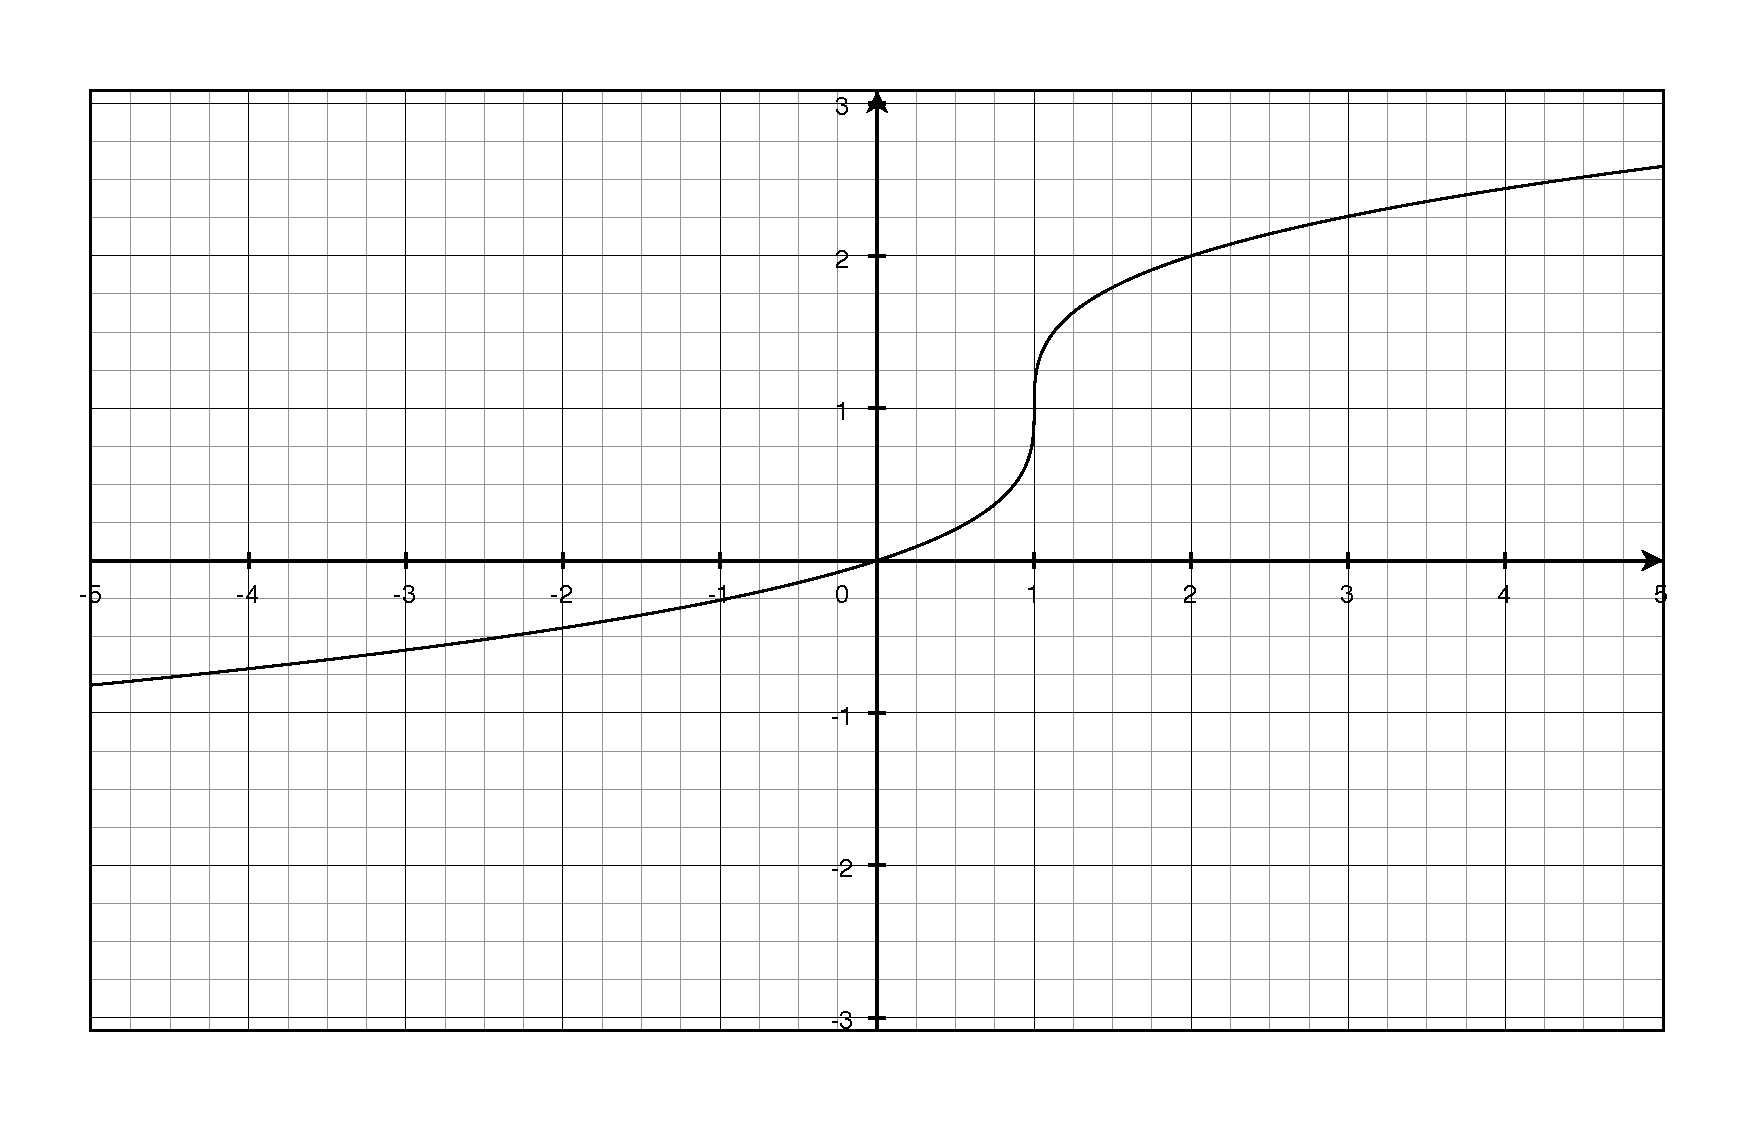
\includegraphics[scale=.3]{question7.eps}
%   \caption*{Question 7}
% \end{figure}

% \begin{tabular}{cc}
% \toprule
% period & amplitude \\
% \midrule
%   $\pi$ & $2$ \\
% \bottomrule
% \end{tabular}

\printanswers

%% \ifprintanswers
%% \usepackage{2in1, lscape}
%% \fi

\title{Math 263A \\ Chapter Four Study Guide \\ Applications}
\date{October 17, 2012}

\author{}

\begin{document}

\maketitle  

\section{Maximum/Minimum}

A value, $c$ is a maximum/minimum in f(x) if $f(c)$ is larger/smaller than all all the other values for $f$ in the region.
The three places maximums and minimums can occur are:

\begin{itemize*}
\item At the end points.
\item At a point where the derivative is zero
\item At a point where the derivative is undefined
\end{itemize*}

When the derivative is zero or undefined the function may be changing direction.  If the derivative is defined and non-zero, then
the functions is increasing or decreasing, so the value can't be a maximum or minimum.

A {\em local min/max}, $c$ is a point where $f(c)$ is smaller/larger than its immediate neighbors but not necessarily
    smaller/larger than all the other points.  If $c$ is a global min/max within a region, $f(c)$ is smaller/larger than $f(x)$ for 
    any value of $x$ in that region.

To find maximums/minimums, first find all the places where the derivative is zero or undefined.  For each of these
points, you need to determine whether the function actually changing direction.  There are two options to do this:
\begin{itemize*}
    \item check whether the second derivative is positive or negative.  A positive second derivative indicates a local minimum
          and a negative second derivative indicates a local maximum.
    \item check whether the first derivative goes from negative to positive or positive to negative at this
          point.  If the function was increasing before and decreasing after, you have a local max, and vice versa.
\end{itemize*}

If you have time, it's a good idea to check both ways.  If they don't agree than you know you made a mistake and you can
go back and correct it.

If you have a closed interval, where the endpoints are included, you also need to check the endpoints to see whether
they are minimums or maximums.

\section{Optimization Problems}
In optimization problems, you are trying to find the ``best'' way to do something, where ``best'' means that you do
something as inexpensively as possible, use the smallest amount of materials, etc.

\subsection{Area/Perimeter}

In an area/perimeter, you are trying to build some sort of usually-oddly-shaped enclosure with some constraint on the
materials used.  Examples are:

\begin{itemize*}
\item build the maximum area pen with an interior divider and a fixed amount of fence
\item build the maximum area rectangular pen with one side provided by a river
\item build the cheapest pen with a specified area and some constraint on the cost of the building materials
\end{itemize*}

To solve this kind of problem:
\begin{itemize*}
\item Draw a picture of the situation.  
\item Label the sides, radius, etc., with variables
\item Get as many equations as you can out of the picture.  The equations may involve cost, area, or perimeter.  Usually
  there will be more than one equation.  One of the equations will always be for the quantity you are trying to minimize
  or maximize.

\item If the equation for the quantity you are trying to maximize has more than one variable in it, you have a problem.
  You can't optimize for two things at once, so you need to get rid of one of the variables.  Do this by:
  \begin{itemize*}
    \item solve another equation for a variable you'd like to get rid of
    \item substitute the result in the first equation  
  \end{itemize*}

\end{itemize*}

Now you have an equation for the quantity you are interested with one variable, and the hard part is over.  To optimize:
\begin{itemize*}
  \item take the derivative
  \item set the resulting equation to zero
  \item solve
\end{itemize*}

This will give you one or more critical values.  To find if any of the candidates are actually maximums or minimums:
\begin{itemize*}
  \item Plug them in the equation and get values
  \item Plug the value of the ends of the range and get values.  It's possible that the best thing to do, for example,
    is to not use any of the expensive fence and build the enclosure entirely out of cheap fence, or something like
    that.
  \item Whichever of these numbers is best is the answer.
\end{itemize*}

If plugging all the numbers into the equation is difficult and time consuming, you can also use the second derivative
test to see if the critical points are minimums or maximums.

\subsection{Surface Area/Volume}
Another common optimization problem is area/volume.  These problems are often disguised as amount of materials/volume or cost/volume.
Minimizing the amount of materials required to build a container of a particular
shape and specified volume really amounts to minimizing the area of the container, given a desired volume.

Example of this type of problem are:
\begin{itemize*}
  \item Find the dimensions of the minimum cost rectangular box with volume $1 \meter^3$ when the materials used for the top and bottom
    cost twice as much as the materials used for the sides.
  \item Find the dimensions which minimize the amount of metal required to construct a $1 \meter^3$ metal container with a cylindrical base and
    hemispherical top.
\end{itemize*}

The steps for this type of problem are:
\begin{itemize*}
\item Draw a picture of the container.
\item Write equations for the area and volume.  Sometimes you need to think of the container in two pieces and add the
  results together.  For example, if your container is a cylinder with a hemispherical base, write equations for a
  cylinder and for a hemisphere, and add them together.
\item If the area equation involves more than one variable, as it usually does:
  \begin{itemize*} 
    \item solve the volume equation for one of the variables
    \item substitute the result in the area equation
  \end{itemize*} 
\end{itemize*}

\section{Graphing}

Calculus provides some helpful tools for drawing graphs.  There is a checklist of things to do, each of which helps give
you a clearer picture of the final graph.  Some of the things you already know from pre-calculus.  Here's the full list:

\subsection{Symmetry}

To determine if there is any symmetry, find $f(-x)$.  

If $f(-x) = f(x)$, the function is {\em even} and has y-axis symmetry.  This is nice because you only need to draw the right
half of the graph.  The left half will be a reflection of the right.

If $f(-x) = -f(x)$, the function is {\em odd} and has origin symmetry.

If neither of these is true, which is usually the case, there isn't any symmetry.

\subsection{First Derivative Test}
\label{first-derivative-test}

Find $f'(x)$ and figure out where it is 0, undefined, negative, and positive.  

The points where $f'(x) = 0$ are {\em critical points}.  These are places where the function might change direction.
The points where $f'(x)$ is undefined are points where either $f(x)$ is undefined, or where $f(x)$ makes a sharp point
or vertical line.  These are also places where the function might change direction.

Critical points are also potential minimums and maximums for the function.  You can determine if one of these values is
actually a minimum or maximum by either:

\begin{itemize*}
  \item If $f'(x)$ has different signs before and after the point, it is a minimum or maximum
  \item If $f''(x) \neq 0$ at this point, it is either a minimum or maximum.  A positive second derivative indicates a
    minimum and a negative second derivative indicates a maximum.
\end{itemize*}

Where $f'(x) > 0$ the original function is increasing.

Where $f'(x) < 0$ the original function is increasing.

\subsection{Second Derivative Test}

Find $f''(x)$ and figure out where it is 0, undefined, negative, and positive.  

The points where $f'(x) = 0$ are {\em inflection points}.  These are places where the function might change shape.

The points where $f''(x)$ is undefined are points where either $f'(x)$ is undefined, or where $f'(x)$ makes a sharp point
or vertical line.  These are also places where the function might change shape.

Where $f''(x) > 0$ the original function is {\em concave up}.

Where $f''(x) < 0$ the original function is {\em concave down}.

The second derivative is also useful in identifying minimums and maximums as described in Section \ref{first-derivative-test}.

\section{Limits at Infinity}
If $\lim_{x \to \pm \infty} = c$, then there is a horizontal asymptote at $c$.

For rational functions, there are several cases for limits at infinity:
\begin{enumerate*}
  \item If the degree of the numerator is greater than the degree of the denominator, the numerator grows much faster
    than the denominator and the limit is infinity.  

  \item If the degree of the denominator is greater than the degree of the numerator, the denominator grows much faster
    than the numerator and the limit is zero.

  \item If the degree of the numerator is equal to the degree of the denominator, they both grow at approximately the
    same rate.  As $x$ gets larger and larger, the terms other than the first term have less and less of an effect on
    the value.  So the limit when the numerator and denominator are equal is the ratio of the coefficients of the
    highest order terms.
\end{enumerate*}

\begin{description}
  \item[case 1] $\lim_{x \to \infty} \frac{x^2}{x + 1} = \infty$
  \item[case 2] $\lim_{x \to \infty} \frac{x^2 + 1}{2x^3 + 3} = 0$
  \item[case 3] $\lim_{x \to \infty} \frac{4x^2 + 3x + 7}{2x^2 - 9} = 2$
\end{description}

To evaluate these limits, divide both numerator and denominator by $x^{max \ exponent}$:
\[
  \lim_{x \to \infty} \frac{4x^2 + 3x + 7}{2x^2 - 9} = \lim_{x \to \infty} \frac{4 + 3/x + 7/x^2}{2 - 9/x^2} 
    = \frac{4}{2} = 2
\]

If the degree of the numerator is exactly one more than the degree of the denominator, the graph will have a {\em slant}
(or {\em oblique}, if you prefer) asymptote.  To find the oblique asymptote, use polynomial long division to divide the
numerator by the denominator.  The quotient will be the equation of a straight line which is the {\em slant} asymptote.

\section{Infinite Limits}
If $\lim_{x \to c} = \pm \infty$ then there is a vertical asymptote at $c$.

\subsection{Drawing the Graph}
Once you have done all the preceding steps, you should have a fairly good picture of the graph.  Select a few key
points, plug the x values into the graph to get the y-values, and draw the graph.

When you are doing this, make sure that the values agree with the shapes, min/max, etc. that you found from earlier
steps.  If they don't agree, something is wrong---go back and check your earlier work and find the problem.


\end{document}
